
%------------------------------------------------

\section{Expectation operation}\index{expectation}
\label{sec:exp_value}

Let $g(x)$ be some function of a random variable $x$ with density $f(x)$.

The expectation of $g(x)$ is the number:

\marginnote[6pt]{The expectation is a linear operation:

$$
\mathrm{E}\left[ a g(x) + b h(x) \right] = a \mathrm{E}\left( g \right) + b \mathrm{E}\left( h \right)
$$
}

\begin{equation}\label{eq:exp_value}
	\mathrm{E}\left( g \right) = \int_{\Omega} {g(x) f(x)} \,\mathrm{d}x
\end{equation} 

\subsection{Mean or average}\index{mean}\index{average}
\label{subsec:mean}

The average is the expectation of the variable itself:

\begin{equation}\label{eq:mean}
	\left \langle x \right \rangle = \bar{x} = \int {x f(x)}\mathrm{d}x
\end{equation}

In the discrete case:

\begin{equation}\label{eq:mean_discrete}
	\left \langle x \right \rangle = \bar{x} = \sum_{i = 1}^{n}{x_{i} P(x_{i})}
\end{equation}

\subsection{Variance}\index{variance}
\label{subsec:variance}

\begin{equation}\label{eq:variance}
	\mathrm{V} = \mathrm{V}\left( x \right) = \sigma^{2} = \mathrm{E}\left[ (x - \bar{x})^{2} \right] 
	= \int {(x - \bar{x})^{2} f(x)}\mathrm{d}x
	= \left \langle x^{2} \right \rangle - {\left \langle x \right \rangle}^2
\end{equation}

In the discrete case:

\begin{equation}\label{eq:variance_discrete}
	\mathrm{V} = \sum_{i = 1}^{n}{(x_{i} - \bar{x})^{2} P(x_{i})}
\end{equation}

\subsection{Standard deviation}\index{standard deviation}
\label{subsec:std_deviation}

\begin{equation}\label{eq:std_deviation}
	\sigma = \sqrt{\mathrm{V}}
\end{equation}

\subsection{Root mean square}\index{root mean square}
\label{subsec:rms}

\marginnote[6pt]{Sometimes people denote $\sigma$ as $\mathrm{rms}$.}

\begin{equation}\label{eq:rms}
	x_{\mathrm{rms}} = \sqrt{\frac{1}{n}\sum_{i=1}^{n}{{x_{i}}^{2}} P(x_{i})} 
	= \sqrt{\left \langle x^{2} \right \rangle}
\end{equation} 

\subsection{Covariance}\index{covariance}
\label{subsec:cov}

Take two variables $x$, $y$ with PDF $f(x, y)$. The covariance is defined as:

\begin{equation}\label{eq:cov}
	\mathrm{cov}\left( x, y \right) = \mathrm{E}\left[ (x - \bar{x}) (y - \bar{y}) \right] 
	= \mathrm{E}\left( xy \right) - \mathrm{E}\left( x \right) \mathrm{E}\left( y \right) 
\end{equation}

where: 

\begin{equation}
	\mathrm{E}\left( xy \right) = \int {xy f(x, y)}\mathrm{d}x \mathrm{d}y
\end{equation}

\begin{equation}
	\mathrm{E}\left( x \right) = \int {x f(x, y)}\mathrm{d}x \mathrm{d}y
\end{equation}

\subsection{Correlation}\index{correlation}
\label{subsec:corr}

\marginnote[6pt]{Always between -1 and 1.}

\begin{equation}\label{eq:corr}
	\mathrm{corr}\left( x, y \right) = \rho_{x, y} = \frac{\mathrm{cov}\left( x, y \right)}{\sigma_{x} \sigma_{y}}
\end{equation} 

where:

\begin{equation}
	{\sigma_{x}}^{2} = \mathrm{E}\left[ (x - \bar{x})^{2} \right]
\end{equation}

\newthought{If} $x$ and $y$ are independent, we have:

\begin{equation}
	\mathrm{E}\left( xy \right) = \int {xy f_{x}(x) f_{y}(y)}\mathrm{d}x \mathrm{d}y 
	= \int {x f_{x}(x)}\mathrm{d}x \int {y f_{y}(y)}\mathrm{d}y 
	= \mathrm{E}\left( x \right) \mathrm{E}\left( y \right)
\end{equation}

Therefore, \mono{independent variables have null covariance and correlation}.

\newthought{Notice}, however, that uncorrelated variables are not necessarily independent!

This is for example the case (Figure~\ref{fig:uncorrelated_4_Gaussian}) of:

\begin{equation}
	f(x, y) = \frac{1}{4} \left[ 
	g(x; \mu, \sigma) g(y; 0, \sigma) + g(x; -\mu, \sigma) g(y; 0, \sigma)
	+ g(x; 0, \sigma) g(y; \mu, \sigma) + g(x; 0, \sigma) g(y; -\mu, \sigma)
	\right]
\end{equation}

\begin{figure}
	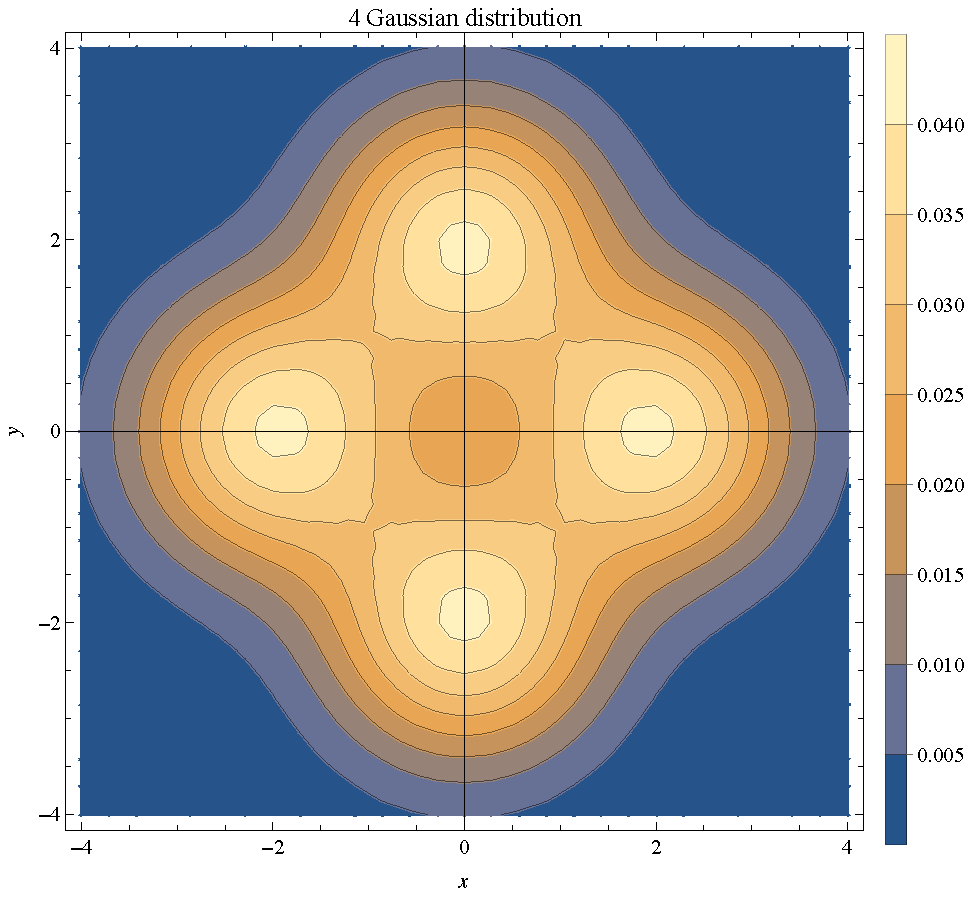
\includegraphics{probability/uncorrelated_4_Gaussian.pdf}
	\caption[4 Gaussian distribution.][6pt]{4 Gaussian distribution.}
	\label{fig:uncorrelated_4_Gaussian}
\end{figure}

\newpage

\subsection{Centroids of a distribution}\index{centroid}
\label{subsec:centroid}

\newthought{Mean}:\index{mean}

\begin{equation}
	\bar{x} = \int {x f(x)}\mathrm{d}x
\end{equation}

\newthought{Mode}:\index{mode}

\begin{equation}\label{eq:mode}
	\hat{x} = \max_{x}(f(x))
\end{equation}

\newthought{Median}:\index{median}

\begin{equation}\label{eq:median}
	\tilde{x} = x: \ P(x < \tilde{x}) = P(x > \tilde{x}) 
	= x: \ \int_{-\infty}^{\tilde{x}} {f(x)} \,\mathrm{d}x 
	= x: \ \int_{\tilde{x}}^{\infty} {f(x)} \,\mathrm{d}x 
	= 0.5
\end{equation}

\newthought{Notice} that mean, mode and median coincide for a symmetric distribution, but \emph{not} for an asymmetric one! (Figure~\ref{fig:mean_mode_median_chisquare})

\begin{figure*}[h]\index{chi-square distribution}
	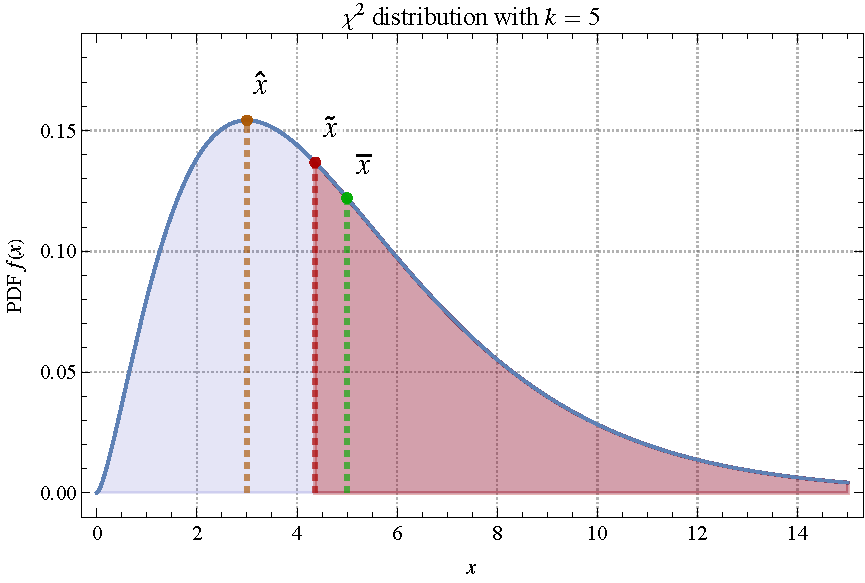
\includegraphics[width=\linewidth]{probability/mean_mode_median_chisquare.pdf}
	\caption[$\chi^{2}$ distribution with $k = 5$.]{$\chi^{2}$ distribution with $k = 5$.}
	\label{fig:mean_mode_median_chisquare}
\end{figure*}

\subsection{Quantiles}\index{quantile}
\label{subsec:quantile}

The quantity $q_{\alpha}$ such that:

\begin{equation}\label{eq:alpha_quantile}
	\int_{-\infty}^{q_{\alpha}} {f(x)} \,\mathrm{d}x = \alpha 
	= 1 - \int_{q_{\alpha}}^{\infty} {f(x)} \,\mathrm{d}x
\end{equation}

is called $\alpha$-quantile.

An alternative definition can be given with the cumulative distribution\index{cumulative distribution}:

\begin{equation}
	q_{\alpha} = x : \ F(x) = \alpha
\end{equation}